\documentclass{article}
\usepackage{graphicx}
\usepackage{float}
\usepackage{epstopdf}

\begin{document} 
\begin{center}
{\bf \Large  Homework 6} \\
\end{center}
Chien-Pin Chen
05/20/2016


\noindent The state of a body falling vertically through the atmosphere is $\underline{\bf \rm x}=[x\ {\dot x}\ \beta]^T$, 
where $x$ is its height above the Earth's surface and $\beta$ its ballistic coefficient. The ballistic coefficient is included as a state because it is not well known,  so it must be estimated. Use EKF for continuous time models and discrete observations.

The state equations are
\begin{eqnarray}
   \frac{d x}{dt} &=& \dot x \\
   \frac{d {\dot x}}{dt} &=& d-g \\
   \frac{d \beta}{dt} &=& \xi(t)
\end{eqnarray}
 where $g=9.8\  [m/s^2]$ is acceleration due to gravity, $\xi(t)$ is the zero-mean white noise of intensity $1000\  [g^2/(m^2 s^6)]$, 
and the drag is given by 
\begin{equation}
  d= \frac{\rho {\dot x}^2}{2 \beta}
\end{equation}
Units are provided in the rectangular brackets, however the problem is defined so that you do not need to worry about them. 

Atmospheric density is 
\begin{equation}
  \rho = \rho_0 e^{- x /c}
\end{equation}
with $\rho_0=1220\  [g/m^3]$ being the density at sea level and $c=10263\  [m]$ a decay constant.

Suppose range measurements are taken every second (T=1\  [s]) as in the figure (see the next page). Thus, 
\begin{equation}
  z_k=\sqrt{r_1^2+(x_k-r_2)^2 }+ v_k
\end{equation}
with $r_1=1000\  [m]$, $r_2=500\ [m]$,  $x_k=x(kT)$ and $v_k \sim N(0,\sigma^2_r)$,  $\sigma_r^2=5\  [m^2]$.\\


\noindent {\bf (a)} Write down the prediction step of EKF; {\bf (b)} Write down the update step of EKF;  {\bf (c)} Assume that at $t=0$, $E\{ x(0)\}=10000[m]$, $var\{ x(0)\}=50[m^2]$,  $E\{{\dot  x}(0)\}=-500[m/s]$, 
 $var\{ {\dot x}(0)\}=200[m^2/s^2]$, $E\{\beta(0)\}=6 \times 10^7 [g/ms^2]$, 
$var(\beta(0))=2 \times 10^{12} [g^2/m^2 s^4]$ and that the measured data are taken every second 
beginning at $t_1=1[s]$, and are given in meters by 
\begin{equation}
z_1,z_2,....z_{10}= 9055, 8560, 7963, 7467, 7000, 6378, 5885, 5400, 4928, 4503
\end{equation}
Plot the $x_m(k)=\sqrt{z_k^2-r_1^2}+r_2$ and the EKF estimates for $x(t)$ on the same 
diagram. On separate diagrams, plot the velocity ($\dot x$) and the ballistic coefficient ($\beta$) estimates. 


\bf{ANS:}\\
For equation 1, I can rewrite as:
\begin{equation}
\frac{d}{{dt}}\left[ {\begin{array}{*{20}c}
   x  \\
   {\dot x}  \\
   \beta   \\
\end{array}} \right] = \left[ {\begin{array}{*{20}c}
   {\dot x}  \\
   {\frac{{\rho _0 e^{ - x/c} \dot x^2 }}{{2\beta }}}  \\
   0  \\
\end{array}} \right] + \left[ {\begin{array}{*{20}c}
   0  \\
   { - g}  \\
   0  \\
\end{array}} \right] + \left[ {\begin{array}{*{20}c}
   0  \\
   0  \\
   {\xi (t)}  \\
\end{array}} \right]
\end{equation}
In Extend Kalman Filter, equation 1 could refer to:
\begin{equation}
    dx=f(x,t)dt+b(t)dw+u\\
\end{equation}
then, for computing, I could set:
\begin{equation}
	f(x,t) = \left[ {\begin{array}{*{20}c}
	   {\dot x}  \\
	   {\frac{{\rho _0 e^{ - x/c} \dot x^2 }}{{2\beta }}}  \\
	   0  \\
	\end{array}} \right],{\rm{  u = }}\left[ {\begin{array}{*{20}c}
	   0  \\
	   { - g}  \\
	   0  \\
	\end{array}} \right]
\end{equation}
Because $\xi (t)$ is the zero-mean white noise of intensity $1000\  [g^2/(m^2 s^6)]$, matrix $b(t)$ could set as:
\begin{equation}
	b = \left[ {\begin{array}{*{20}c}
	   0  \\
	   0  \\
	   {\sqrt {1000} }  \\
	\end{array}} \right]
\end{equation}
And, equation 2 can refer to the equation in discrete observation step:
\begin{equation}
	\underline{y}(t_k)=\underline{h_k}(\underline{x}(t_k))+\underline{v}(t_k)
\end{equation}

\noindent \textbf{a.} In the prediction step of EKF:\\
I use following equations and compute with MATLAB ode45 function for continuous time model:
\begin{eqnarray}
	\underline{\dot{\hat{x}}}(t) = f(\underline{\hat{x}},t) + u{\rm{  }}t \in \left[ {t_k ,t_{k + 1} } \right]\\
	\underline{\dot{A}} (t) = \frac{{\partial f(\underline{\hat{x}},t)}}{{\partial \underline{\hat{x}}}} = \left[ {\begin{array}{*{20}c}
	   0 & 1 & 0  \\
	   { - \frac{{\rho _0 e^{ - x/c} \dot x^2 }}{{2\beta c}}} & {\frac{{\rho _0 e^{ - x/c} \dot x}}{\beta }} & { - \frac{{\rho _0 e^{ - x/c} \dot x^2 }}{{2\beta ^2 }}}  \\
	   0 & 0 & 0  \\
	\end{array}} \right]\\
	\underline{\dot{P}} (t) = \underline{A} (t)P(t) + P(t)\underline{A}^T (t) + bb^T (t),{\rm{ }}t \in [t_k ,t_{k + 1} ]
\end{eqnarray}
For initial guess of $\underline{\hat{x}}_0$, I use expected value provided in (c) part:
\begin{equation}
	\underline{\hat{x}}0  = \left[ {\begin{array}{*{20}c}
	   {E\{ x(0)\} }  \\
	   {E\{ \dot x(0)\} }  \\
	   {E\{ \beta (0)\} }  \\
	\end{array}} \right] = \left[ {\begin{array}{*{20}c}
	   {10000}  \\
	   { - 500}  \\
	   {6 \times 10^7 }  \\
	\end{array}} \right]
\end{equation}
For initial guess of $\underline{\hat{P}}_0$, I use variance value provided in (c) part:
\begin{equation}
\underline{\hat{P}}_0  = \left[ {\begin{array}{*{20}c}
   {{\mathop{\rm var}} \{ x(0)\} } & {P_{12} } & {P_{13} }  \\
   {P_{21} } & {{\mathop{\rm var}} \{ \dot x(0)\} } & {P_{23} }  \\
   {P_{31} } & {P_{32} } & {{\mathop{\rm var}} \{ \beta (0)\} }  \\
\end{array}} \right]{\rm{ = }}\left[ {\begin{array}{*{20}c}
   {50} & 0 & 0  \\
   0 & {200} & 0  \\
   0 & 0 & {2 \times 10^{12} }  \\
\end{array}} \right]
\end{equation}
In my computing, the covriance element of  $\underline{\hat{P}}_0$ are set to zero for simplified.
After doing ode45 function, ode45 function will return two sequence of the result (time and array of $\underline{\hat{x}}(t_{k+1}), \underline{P}(t_{k+1})$ ), and
I will assign the last array in the sequence as the prediction of EKF:
\begin{equation}
\begin{array}{l}
\underline{\hat{x}}_{k + 1} ( - ) = \underline{\hat{x}}(t_{k + 1} ) \\ 
 \underline{\hat{P}}_{k + 1} ( - ) = \underline{\hat{P}}(t_{k + 1} ) \\ 
 \end{array}
\end{equation}  

\noindent \textbf{b.}  In the prediction step of EKF:\\
First, I use $\underline{\hat{x}}(t_{k+1})$ to update $\underline{H}_{k+1}$:
\begin{equation}
	\underline{H}_{k + 1}  = \frac{{\partial h_{k + 1} (x_{k + 1} ( - ))}}{{\partial x_{k + 1} }} = \frac{{(x_k  - r_2 )}}{{\sqrt {r_1^2  + (x_k  - r_2 )} }}
\end{equation}
Then, I use the new $\underline{H}_{k+1}$ to compute the new kalman filter gain:
\begin{equation}
	\underline{H}_{k + 1}  = \underline{P}_{K + 1} ( - )\underline{H}_{k + 1}^T (\underline{H}_{k + 1} \underline{P}_{K + 1} ( - )\underline{H}_{k + 1}^T  + \underline{R}_{k + 1} )^{ - 1} 
\end{equation} 
with new $\underline{H}_{k+1}$ and $\underline{K}_k+1$, I can update $\underline{\hat{x}}_{k+1}$ and $\underline{P}_{k+1}$:
\begin{equation}
\begin{array}{l}
 \underline{\hat{x}}_{k + 1}  = \underline{\hat{x}}_{k + 1} ( - ) + \underline{K}_{k + 1} (\underline{y}_{k + 1}  - \underline{h}_{k + 1} (\underline{\hat{x}}_{k + 1} ( - ))) \\ 
 \underline{P}_{k + 1}  = (I - \underline{K}_{k + 1} \underline{H}_{k + 1} )\underline{P}_{k + 1} ( - ) \\ 
 \end{array}
\end{equation}
After updating, do another extend kalman filter with next measurement $z_k$.\\
\noindent \textbf{c.}\\
First, I use $x_m(k)=\sqrt{z_k^2-r_1^2}+r_2$ with $z_k$ to get the sequence of $x_m$.
In all figures, I also add cumulating results of $x(t)$ from ode45 (as green line).
The following is the diagram of $x_m$ and $E{x(t_k)}$:
\begin{figure}[H]
\begin{center}
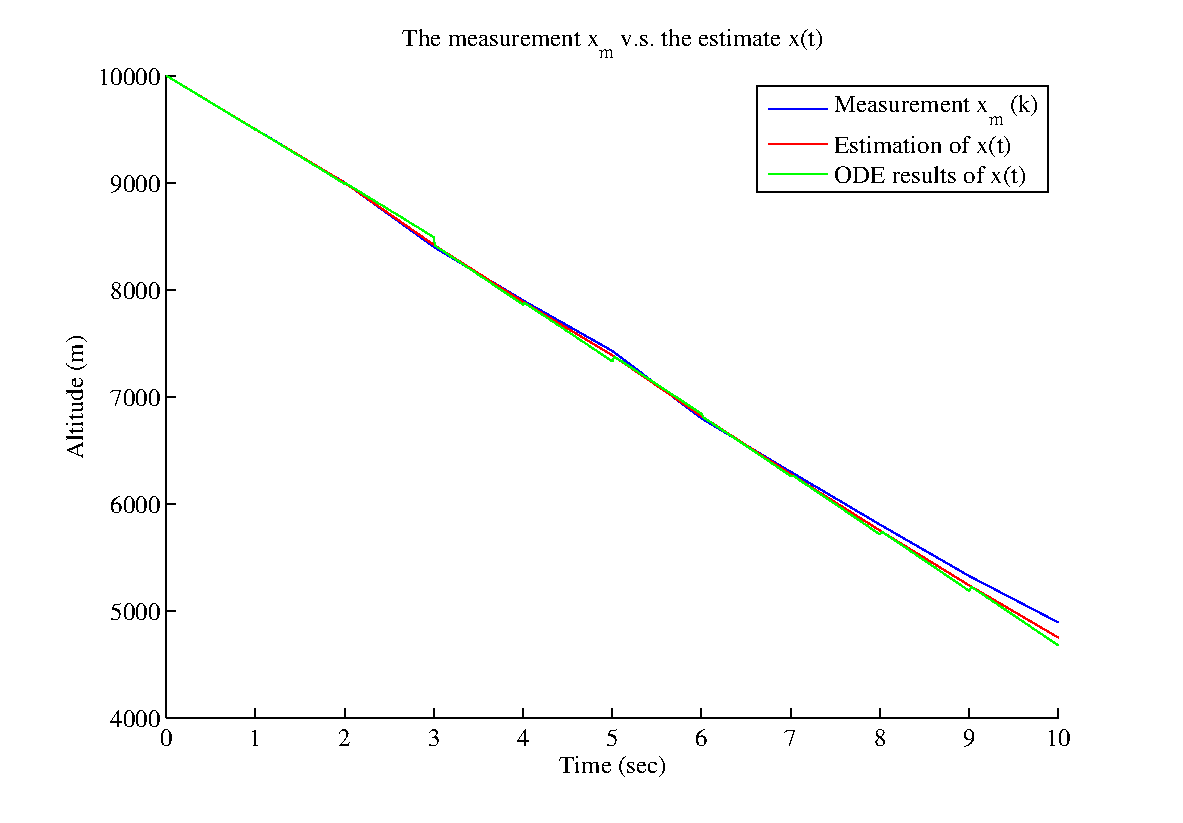
\includegraphics[width=\textwidth]{hw6_xmxt.eps}
\caption{The measurement $x_m$ and the EKF estimate x(t).}
\end{center}
\end{figure} 
\pagebreak 
The following is the diagram for the velocity $\dot{x}(t)$:
\begin{figure}[H]
\begin{center}
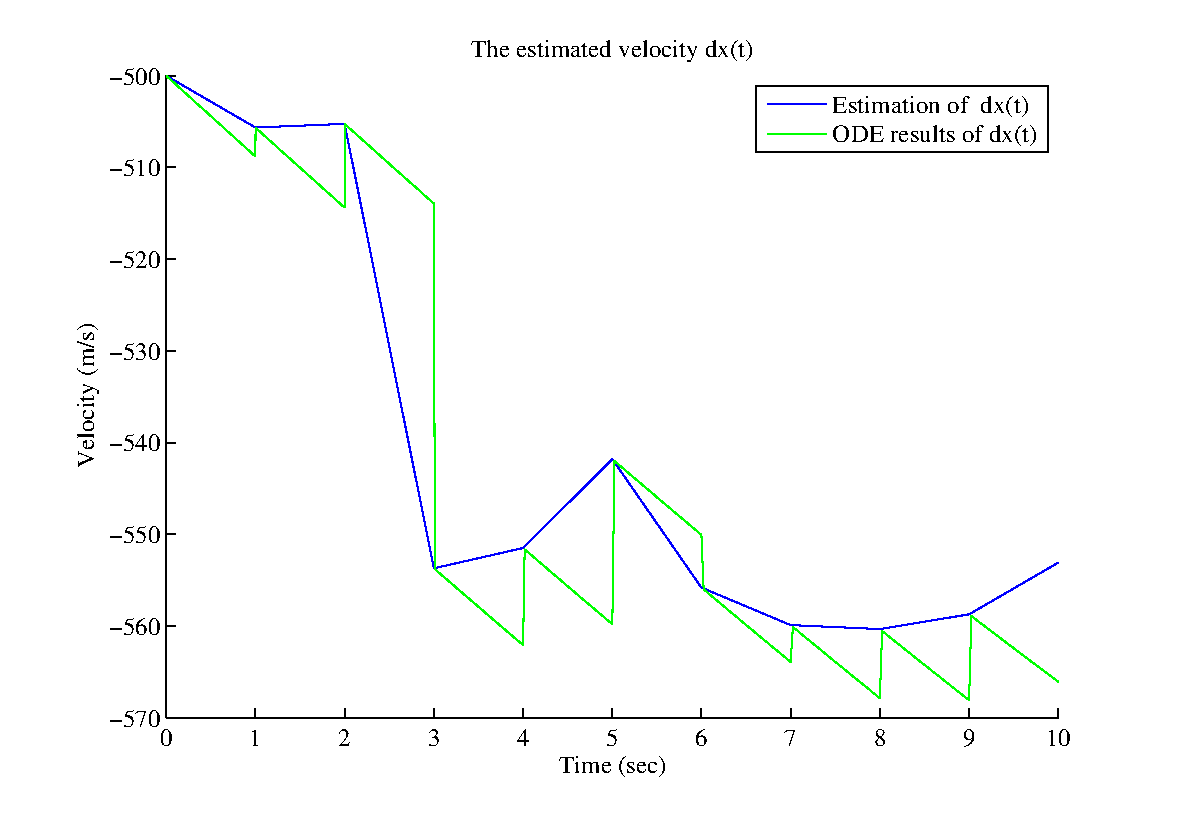
\includegraphics[width=\textwidth]{hw6_dx.eps}
\caption{ The EKF estimate $\dot{x}(t)$.}
\end{center}
\end{figure} 
\pagebreak 
The following is the diagram for the ballistic coefficient $\beta(t)$:
\begin{figure}[H]
\begin{center}
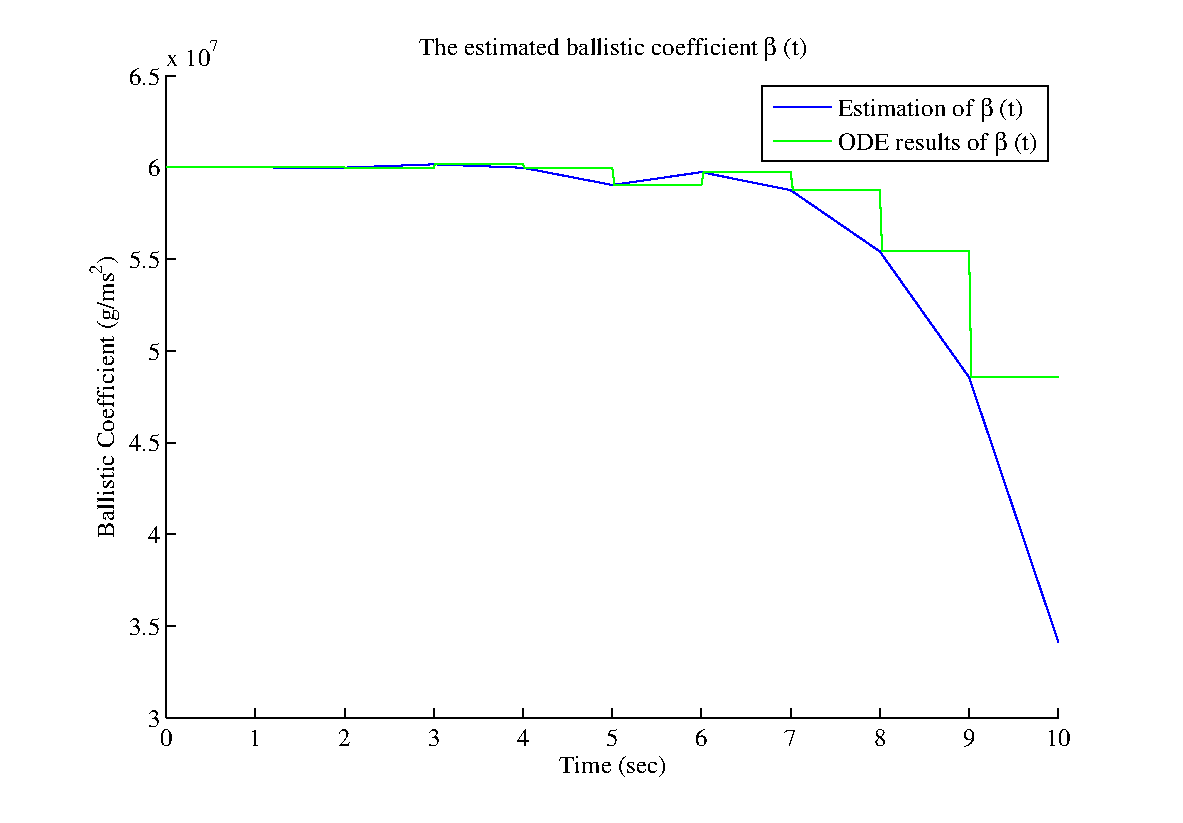
\includegraphics[width=\textwidth]{hw6_beta.eps}
\caption{ The EKF estimate $\beta(t)$.}
\end{center}
\end{figure} 

\end{document}
